\documentclass[1p]{elsarticle_modified}
%\bibliographystyle{elsarticle-num}

%\usepackage[colorlinks]{hyperref}
%\usepackage{abbrmath_seonhwa} %\Abb, \Ascr, \Acal ,\Abf, \Afrak
\usepackage{amsfonts}
\usepackage{amssymb}
\usepackage{amsmath}
\usepackage{amsthm}
\usepackage{scalefnt}
\usepackage{amsbsy}
\usepackage{kotex}
\usepackage{caption}
\usepackage{subfig}
\usepackage{color}
\usepackage{graphicx}
\usepackage{xcolor} %% white, black, red, green, blue, cyan, magenta, yellow
\usepackage{float}
\usepackage{setspace}
\usepackage{hyperref}

\usepackage{tikz}
\usetikzlibrary{arrows}

\usepackage{multirow}
\usepackage{array} % fixed length table
\usepackage{hhline}

%%%%%%%%%%%%%%%%%%%%%
\makeatletter
\renewcommand*\env@matrix[1][\arraystretch]{%
	\edef\arraystretch{#1}%
	\hskip -\arraycolsep
	\let\@ifnextchar\new@ifnextchar
	\array{*\c@MaxMatrixCols c}}
\makeatother %https://tex.stackexchange.com/questions/14071/how-can-i-increase-the-line-spacing-in-a-matrix
%%%%%%%%%%%%%%%

\usepackage[normalem]{ulem}

\newcommand{\msout}[1]{\ifmmode\text{\sout{\ensuremath{#1}}}\else\sout{#1}\fi}
%SOURCE: \msout is \stkout macro in https://tex.stackexchange.com/questions/20609/strikeout-in-math-mode

\newcommand{\cancel}[1]{
	\ifmmode
	{\color{red}\msout{#1}}
	\else
	{\color{red}\sout{#1}}
	\fi
}

\newcommand{\add}[1]{
	{\color{blue}\uwave{#1}}
}

\newcommand{\replace}[2]{
	\ifmmode
	{\color{red}\msout{#1}}{\color{blue}\uwave{#2}}
	\else
	{\color{red}\sout{#1}}{\color{blue}\uwave{#2}}
	\fi
}

\newcommand{\Sol}{\mathcal{S}} %segment
\newcommand{\D}{D} %diagram
\newcommand{\A}{\mathcal{A}} %arc


%%%%%%%%%%%%%%%%%%%%%%%%%%%%%5 test

\def\sl{\operatorname{\textup{SL}}(2,\Cbb)}
\def\psl{\operatorname{\textup{PSL}}(2,\Cbb)}
\def\quan{\mkern 1mu \triangleright \mkern 1mu}

\theoremstyle{definition}
\newtheorem{thm}{Theorem}[section]
\newtheorem{prop}[thm]{Proposition}
\newtheorem{lem}[thm]{Lemma}
\newtheorem{ques}[thm]{Question}
\newtheorem{cor}[thm]{Corollary}
\newtheorem{defn}[thm]{Definition}
\newtheorem{exam}[thm]{Example}
\newtheorem{rmk}[thm]{Remark}
\newtheorem{alg}[thm]{Algorithm}

\newcommand{\I}{\sqrt{-1}}
\begin{document}

%\begin{frontmatter}
%
%\title{Boundary parabolic representations of knots up to 8 crossings}
%
%%% Group authors per affiliation:
%\author{Yunhi Cho} 
%\address{Department of Mathematics, University of Seoul, Seoul, Korea}
%\ead{yhcho@uos.ac.kr}
%
%
%\author{Seonhwa Kim} %\fnref{s_kim}}
%\address{Center for Geometry and Physics, Institute for Basic Science, Pohang, 37673, Korea}
%\ead{ryeona17@ibs.re.kr}
%
%\author{Hyuk Kim}
%\address{Department of Mathematical Sciences, Seoul National University, Seoul 08826, Korea}
%\ead{hyukkim@snu.ac.kr}
%
%\author{Seokbeom Yoon}
%\address{Department of Mathematical Sciences, Seoul National University, Seoul, 08826,  Korea}
%\ead{sbyoon15@snu.ac.kr}
%
%\begin{abstract}
%We find all boundary parabolic representation of knots up to 8 crossings.
%
%\end{abstract}
%\begin{keyword}
%    \MSC[2010] 57M25 
%\end{keyword}
%
%\end{frontmatter}

%\linenumbers
%\tableofcontents
%
\newcommand\colored[1]{\textcolor{white}{\rule[-0.35ex]{0.8em}{1.4ex}}\kern-0.8em\color{red} #1}%
%\newcommand\colored[1]{\textcolor{white}{ #1}\kern-2.17ex	\textcolor{white}{ #1}\kern-1.81ex	\textcolor{white}{ #1}\kern-2.15ex\color{red}#1	}

{\Large $\underline{12n_{0544}~(K12n_{0544})}$}

\setlength{\tabcolsep}{10pt}
\renewcommand{\arraystretch}{1.6}
\vspace{1cm}\begin{tabular}{m{100pt}>{\centering\arraybackslash}m{274pt}}
\multirow{5}{120pt}{
	\centering
	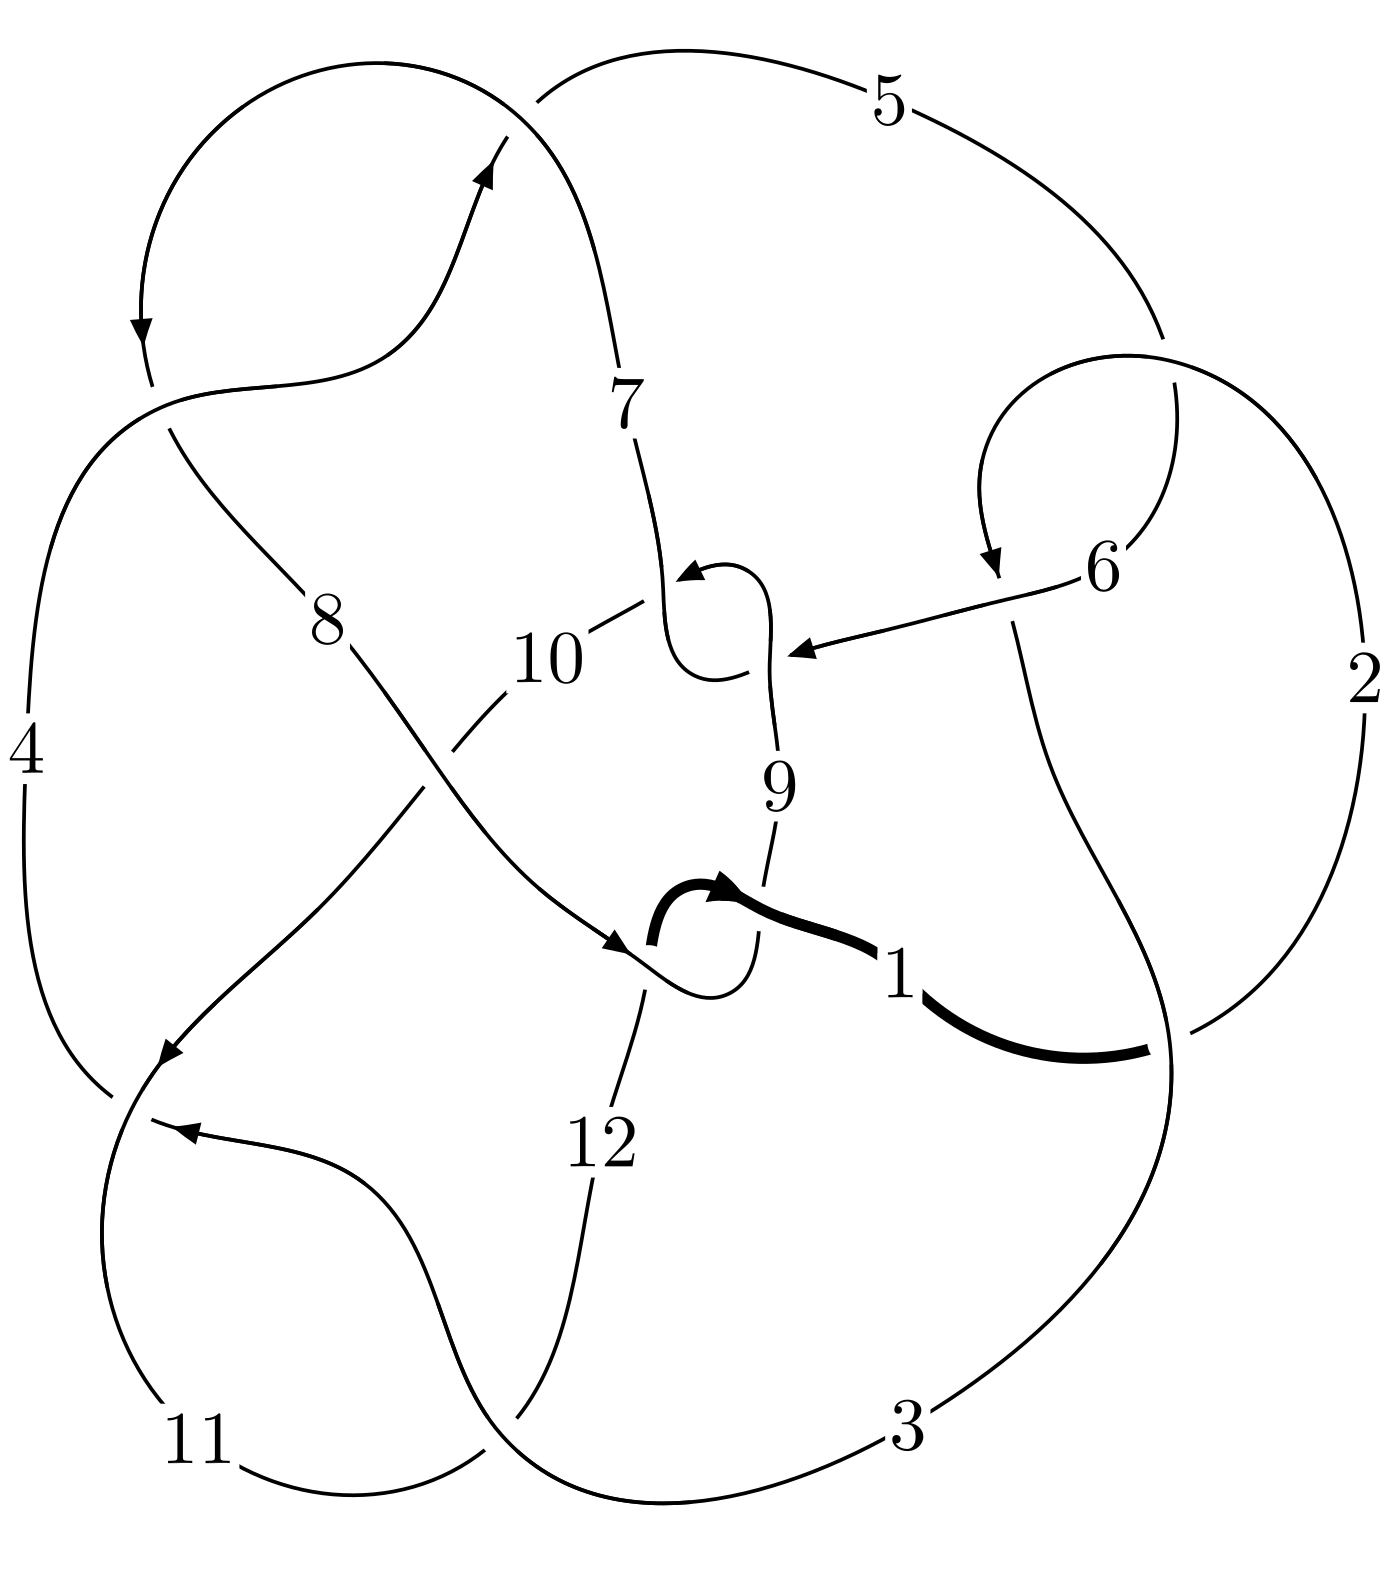
\includegraphics[width=112pt]{../../../GIT/diagram.site/Diagrams/png/2633_12n_0544.png}\\
\ \ \ A knot diagram\footnotemark}&
\allowdisplaybreaks
\textbf{Linearized knot diagam} \\
\cline{2-2}
 &
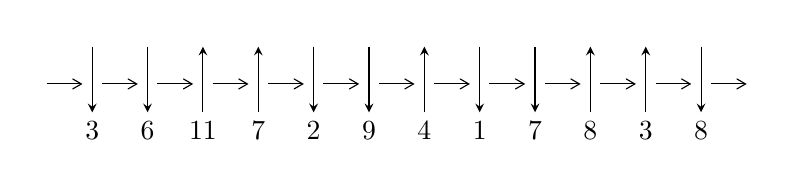
\begin{tikzpicture}[x=20pt, y=17pt]
	% nodes
	\node (C0) at (0, 0) {};
	\node (C1) at (1, 0) {};
	\node (C1U) at (1, +1) {};
	\node (C1D) at (1, -1) {3};

	\node (C2) at (2, 0) {};
	\node (C2U) at (2, +1) {};
	\node (C2D) at (2, -1) {6};

	\node (C3) at (3, 0) {};
	\node (C3U) at (3, +1) {};
	\node (C3D) at (3, -1) {11};

	\node (C4) at (4, 0) {};
	\node (C4U) at (4, +1) {};
	\node (C4D) at (4, -1) {7};

	\node (C5) at (5, 0) {};
	\node (C5U) at (5, +1) {};
	\node (C5D) at (5, -1) {2};

	\node (C6) at (6, 0) {};
	\node (C6U) at (6, +1) {};
	\node (C6D) at (6, -1) {9};

	\node (C7) at (7, 0) {};
	\node (C7U) at (7, +1) {};
	\node (C7D) at (7, -1) {4};

	\node (C8) at (8, 0) {};
	\node (C8U) at (8, +1) {};
	\node (C8D) at (8, -1) {1};

	\node (C9) at (9, 0) {};
	\node (C9U) at (9, +1) {};
	\node (C9D) at (9, -1) {7};

	\node (C10) at (10, 0) {};
	\node (C10U) at (10, +1) {};
	\node (C10D) at (10, -1) {8};

	\node (C11) at (11, 0) {};
	\node (C11U) at (11, +1) {};
	\node (C11D) at (11, -1) {3};

	\node (C12) at (12, 0) {};
	\node (C12U) at (12, +1) {};
	\node (C12D) at (12, -1) {8};
	\node (C13) at (13, 0) {};

	% arrows
	\draw[->,>={angle 60}]
	(C0) edge (C1) (C1) edge (C2) (C2) edge (C3) (C3) edge (C4) (C4) edge (C5) (C5) edge (C6) (C6) edge (C7) (C7) edge (C8) (C8) edge (C9) (C9) edge (C10) (C10) edge (C11) (C11) edge (C12) (C12) edge (C13) ;	\draw[->,>=stealth]
	(C1U) edge (C1D) (C2U) edge (C2D) (C3D) edge (C3U) (C4D) edge (C4U) (C5U) edge (C5D) (C6U) edge (C6D) (C7D) edge (C7U) (C8U) edge (C8D) (C9U) edge (C9D) (C10D) edge (C10U) (C11D) edge (C11U) (C12U) edge (C12D) ;
	\end{tikzpicture} \\
\hhline{~~} \\& 
\textbf{Solving Sequence} \\ \cline{2-2} 
 &
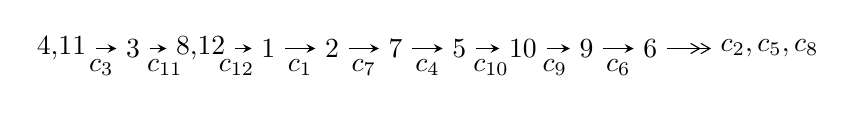
\begin{tikzpicture}[x=23pt, y=7pt]
	% node
	\node (A0) at (-1/8, 0) {4,11};
	\node (A1) at (1, 0) {3};
	\node (A2) at (33/16, 0) {8,12};
	\node (A3) at (25/8, 0) {1};
	\node (A4) at (33/8, 0) {2};
	\node (A5) at (41/8, 0) {7};
	\node (A6) at (49/8, 0) {5};
	\node (A7) at (57/8, 0) {10};
	\node (A8) at (65/8, 0) {9};
	\node (A9) at (73/8, 0) {6};
	\node (C1) at (1/2, -1) {$c_{3}$};
	\node (C2) at (3/2, -1) {$c_{11}$};
	\node (C3) at (21/8, -1) {$c_{12}$};
	\node (C4) at (29/8, -1) {$c_{1}$};
	\node (C5) at (37/8, -1) {$c_{7}$};
	\node (C6) at (45/8, -1) {$c_{4}$};
	\node (C7) at (53/8, -1) {$c_{10}$};
	\node (C8) at (61/8, -1) {$c_{9}$};
	\node (C9) at (69/8, -1) {$c_{6}$};
	\node (A10) at (11, 0) {$c_{2},c_{5},c_{8}$};

	% edge
	\draw[->,>=stealth]	
	(A0) edge (A1) (A1) edge (A2) (A2) edge (A3) (A3) edge (A4) (A4) edge (A5) (A5) edge (A6) (A6) edge (A7) (A7) edge (A8) (A8) edge (A9) ;
	\draw[->>,>={angle 60}]	
	(A9) edge (A10);
\end{tikzpicture} \\ 

\end{tabular} \\

\footnotetext{
The image of knot diagram is generated by the software ``\textbf{Draw programme}" developed by Andrew Bartholomew(\url{http://www.layer8.co.uk/maths/draw/index.htm\#Running-draw}), where we modified some parts for our purpose(\url{https://github.com/CATsTAILs/LinksPainter}).
}\phantom \\ \newline 
\centering \textbf{Ideals for irreducible components\footnotemark of $X_{\text{par}}$} 
 
\begin{align*}
I^u_{1}&=\langle 
b- u,\;-297940 u^{22}+1271608 u^{21}+\cdots+35873 a-1822970,\;u^{23}- u^{22}+\cdots+2 u-1\rangle \\
I^u_{2}&=\langle 
-3.19561\times10^{118} u^{57}+9.66229\times10^{118} u^{56}+\cdots+3.56639\times10^{118} b+1.16120\times10^{121},\\
\phantom{I^u_{2}}&\phantom{= \langle  }-5.59702\times10^{119} u^{57}+1.70818\times10^{120} u^{56}+\cdots+1.13768\times10^{121} a-1.17564\times10^{123},\\
\phantom{I^u_{2}}&\phantom{= \langle  }u^{58}-3 u^{57}+\cdots-1554 u+319\rangle \\
I^u_{3}&=\langle 
b+u,\;u^{11}-2 u^{10}+6 u^9-9 u^8+14 u^7-14 u^6+15 u^5-10 u^4+8 u^3-4 u^2+a+3 u,\\
\phantom{I^u_{3}}&\phantom{= \langle  }u^{12}- u^{11}+5 u^{10}-4 u^9+10 u^8-5 u^7+11 u^6-2 u^5+8 u^4+u^3+4 u^2+2 u+1\rangle \\
I^u_{4}&=\langle 
- u^9-6 u^7+2 u^6-13 u^5+5 u^4-13 u^3+2 u^2+b-6 u,\;2 u^8+11 u^6-4 u^5+20 u^4-8 u^3+14 u^2+a+u+3,\\
\phantom{I^u_{4}}&\phantom{= \langle  }u^{10}+6 u^8-2 u^7+13 u^6-5 u^5+13 u^4-2 u^3+6 u^2+1\rangle \\
\\
\end{align*}
\raggedright * 4 irreducible components of $\dim_{\mathbb{C}}=0$, with total 103 representations.\\
\footnotetext{All coefficients of polynomials are rational numbers. But the coefficients are sometimes approximated in decimal forms when there is not enough margin.}
\newpage
\renewcommand{\arraystretch}{1}
\centering \section*{I. $I^u_{1}= \langle b- u,\;-2.98\times10^{5} u^{22}+1.27\times10^{6} u^{21}+\cdots+3.59\times10^{4} a-1.82\times10^{6},\;u^{23}- u^{22}+\cdots+2 u-1 \rangle$}
\flushleft \textbf{(i) Arc colorings}\\
\begin{tabular}{m{7pt} m{180pt} m{7pt} m{180pt} }
\flushright $a_{4}=$&$\begin{pmatrix}1\\0\end{pmatrix}$ \\
\flushright $a_{11}=$&$\begin{pmatrix}0\\u\end{pmatrix}$ \\
\flushright $a_{3}=$&$\begin{pmatrix}1\\u^2\end{pmatrix}$ \\
\flushright $a_{8}=$&$\begin{pmatrix}8.30541 u^{22}-35.4475 u^{21}+\cdots-119.158 u+50.8173\\u\end{pmatrix}$ \\
\flushright $a_{12}=$&$\begin{pmatrix}u\\u^3+u\end{pmatrix}$ \\
\flushright $a_{1}=$&$\begin{pmatrix}-6.42670 u^{22}+32.7476 u^{21}+\cdots+118.160 u-51.7962\\2.08212 u^{22}-9.08254 u^{21}+\cdots-29.5331 u+12.6710\end{pmatrix}$ \\
\flushright $a_{2}=$&$\begin{pmatrix}-6.22329 u^{22}+26.3650 u^{21}+\cdots+88.6247 u-38.1463\\2.15839 u^{22}-6.69484 u^{21}+\cdots-16.9712 u+6.49179\end{pmatrix}$ \\
\flushright $a_{7}=$&$\begin{pmatrix}8.30541 u^{22}-35.4475 u^{21}+\cdots-120.158 u+50.8173\\u\end{pmatrix}$ \\
\flushright $a_{5}=$&$\begin{pmatrix}27.1421 u^{22}-24.0277 u^{21}+\cdots-34.2065 u-7.30541\\- u^2\end{pmatrix}$ \\
\flushright $a_{10}=$&$\begin{pmatrix}-3.87484 u^{22}+24.8029 u^{21}+\cdots+100.302 u-45.5822\\3.11435 u^{22}-17.5854 u^{21}+\cdots-61.5896 u+27.1421\end{pmatrix}$ \\
\flushright $a_{9}=$&$\begin{pmatrix}4.63399 u^{22}-17.0272 u^{21}+\cdots-47.3917 u+18.8850\\1.03222 u^{22}-8.50286 u^{21}+\cdots-31.0564 u+14.4711\end{pmatrix}$ \\
\flushright $a_{6}=$&$\begin{pmatrix}-0.909765 u^{22}+6.70869 u^{21}+\cdots+19.6352 u-10.1222\\2.15839 u^{22}-6.69484 u^{21}+\cdots-16.9712 u+6.49179\end{pmatrix}$\\&\end{tabular}
\flushleft \textbf{(ii) Obstruction class $= -1$}\\~\\
\flushleft \textbf{(iii) Cusp Shapes $= -\frac{1000543}{35873} u^{22}-\frac{712577}{35873} u^{21}+\cdots-\frac{3006108}{35873} u+\frac{2311747}{35873}$}\\~\\
\newpage\renewcommand{\arraystretch}{1}
\flushleft \textbf{(iv) u-Polynomials at the component}\newline \\
\begin{tabular}{m{50pt}|m{274pt}}
Crossings & \hspace{64pt}u-Polynomials at each crossing \\
\hline $$\begin{aligned}c_{1}\end{aligned}$$&$\begin{aligned}
&u^{23}+8 u^{22}+\cdots+224 u+64
\end{aligned}$\\
\hline $$\begin{aligned}c_{2},c_{5}\end{aligned}$$&$\begin{aligned}
&u^{23}+8 u^{22}+\cdots-56 u-8
\end{aligned}$\\
\hline $$\begin{aligned}c_{3},c_{4},c_{7}\\c_{11}\end{aligned}$$&$\begin{aligned}
&u^{23}+u^{22}+\cdots+2 u+1
\end{aligned}$\\
\hline $$\begin{aligned}c_{6},c_{8},c_{9}\\c_{12}\end{aligned}$$&$\begin{aligned}
&u^{23}+u^{22}+\cdots- u+1
\end{aligned}$\\
\hline $$\begin{aligned}c_{10}\end{aligned}$$&$\begin{aligned}
&u^{23}+19 u^{22}+\cdots+1792 u+256
\end{aligned}$\\
\hline
\end{tabular}\\~\\
\newpage\renewcommand{\arraystretch}{1}
\flushleft \textbf{(v) Riley Polynomials at the component}\newline \\
\begin{tabular}{m{50pt}|m{274pt}}
Crossings & \hspace{64pt}Riley Polynomials at each crossing \\
\hline $$\begin{aligned}c_{1}\end{aligned}$$&$\begin{aligned}
&y^{23}+4 y^{22}+\cdots-46592 y-4096
\end{aligned}$\\
\hline $$\begin{aligned}c_{2},c_{5}\end{aligned}$$&$\begin{aligned}
&y^{23}-8 y^{22}+\cdots+224 y-64
\end{aligned}$\\
\hline $$\begin{aligned}c_{3},c_{4},c_{7}\\c_{11}\end{aligned}$$&$\begin{aligned}
&y^{23}+9 y^{22}+\cdots-14 y-1
\end{aligned}$\\
\hline $$\begin{aligned}c_{6},c_{8},c_{9}\\c_{12}\end{aligned}$$&$\begin{aligned}
&y^{23}-7 y^{22}+\cdots+7 y-1
\end{aligned}$\\
\hline $$\begin{aligned}c_{10}\end{aligned}$$&$\begin{aligned}
&y^{23}+3 y^{22}+\cdots-917504 y-65536
\end{aligned}$\\
\hline
\end{tabular}\\~\\
\newpage\flushleft \textbf{(vi) Complex Volumes and Cusp Shapes}
$$\begin{array}{c|c|c}  
\text{Solutions to }I^u_{1}& \I (\text{vol} + \sqrt{-1}CS) & \text{Cusp shape}\\
 \hline 
\begin{aligned}
u &= \phantom{-}0.595557 + 0.724305 I \\
a &= \phantom{-}0.588152 + 0.605726 I \\
b &= \phantom{-}0.595557 + 0.724305 I\end{aligned}
 & -3.26156 - 2.02161 I & -7.52324 + 1.29376 I \\ \hline\begin{aligned}
u &= \phantom{-}0.595557 - 0.724305 I \\
a &= \phantom{-}0.588152 - 0.605726 I \\
b &= \phantom{-}0.595557 - 0.724305 I\end{aligned}
 & -3.26156 + 2.02161 I & -7.52324 - 1.29376 I \\ \hline\begin{aligned}
u &= -0.076288 + 0.784165 I \\
a &= -1.76014 - 1.54801 I \\
b &= -0.076288 + 0.784165 I\end{aligned}
 & -4.83015 - 0.57289 I & -12.62080 + 1.94666 I \\ \hline\begin{aligned}
u &= -0.076288 - 0.784165 I \\
a &= -1.76014 + 1.54801 I \\
b &= -0.076288 - 0.784165 I\end{aligned}
 & -4.83015 + 0.57289 I & -12.62080 - 1.94666 I \\ \hline\begin{aligned}
u &= \phantom{-}0.034883 + 0.769214 I \\
a &= -2.73995 - 0.59974 I \\
b &= \phantom{-}0.034883 + 0.769214 I\end{aligned}
 & -3.21113 + 6.60809 I & -8.60360 - 5.54346 I \\ \hline\begin{aligned}
u &= \phantom{-}0.034883 - 0.769214 I \\
a &= -2.73995 + 0.59974 I \\
b &= \phantom{-}0.034883 - 0.769214 I\end{aligned}
 & -3.21113 - 6.60809 I & -8.60360 + 5.54346 I \\ \hline\begin{aligned}
u &= \phantom{-}0.892857 + 0.857700 I \\
a &= \phantom{-}0.995548 - 0.607995 I \\
b &= \phantom{-}0.892857 + 0.857700 I\end{aligned}
 & \phantom{-}2.59080 - 3.50765 I & -2.16401 + 2.34355 I \\ \hline\begin{aligned}
u &= \phantom{-}0.892857 - 0.857700 I \\
a &= \phantom{-}0.995548 + 0.607995 I \\
b &= \phantom{-}0.892857 - 0.857700 I\end{aligned}
 & \phantom{-}2.59080 + 3.50765 I & -2.16401 - 2.34355 I \\ \hline\begin{aligned}
u &= -0.954684 + 0.841112 I \\
a &= -0.696145 + 0.071332 I \\
b &= -0.954684 + 0.841112 I\end{aligned}
 & \phantom{-}0.46179 - 3.67942 I & -15.1455 + 3.7839 I \\ \hline\begin{aligned}
u &= -0.954684 - 0.841112 I \\
a &= -0.696145 - 0.071332 I \\
b &= -0.954684 - 0.841112 I\end{aligned}
 & \phantom{-}0.46179 + 3.67942 I & -15.1455 - 3.7839 I\\
 \hline 
 \end{array}$$\newpage$$\begin{array}{c|c|c}  
\text{Solutions to }I^u_{1}& \I (\text{vol} + \sqrt{-1}CS) & \text{Cusp shape}\\
 \hline 
\begin{aligned}
u &= -0.030245 + 0.711475 I \\
a &= \phantom{-}1.98396 - 0.44610 I \\
b &= -0.030245 + 0.711475 I\end{aligned}
 & -1.04488 - 2.00499 I & -5.60935 + 2.44566 I \\ \hline\begin{aligned}
u &= -0.030245 - 0.711475 I \\
a &= \phantom{-}1.98396 + 0.44610 I \\
b &= -0.030245 - 0.711475 I\end{aligned}
 & -1.04488 + 2.00499 I & -5.60935 - 2.44566 I \\ \hline\begin{aligned}
u &= -0.820681 + 1.010850 I \\
a &= -0.875561 - 0.658608 I \\
b &= -0.820681 + 1.010850 I\end{aligned}
 & \phantom{-}3.30522 - 2.73850 I & -1.61112 + 1.01002 I \\ \hline\begin{aligned}
u &= -0.820681 - 1.010850 I \\
a &= -0.875561 + 0.658608 I \\
b &= -0.820681 - 1.010850 I\end{aligned}
 & \phantom{-}3.30522 + 2.73850 I & -1.61112 - 1.01002 I \\ \hline\begin{aligned}
u &= \phantom{-}0.771841 + 1.092470 I \\
a &= \phantom{-}1.131310 - 0.059859 I \\
b &= \phantom{-}0.771841 + 1.092470 I\end{aligned}
 & -5.97493 + 8.04810 I & -9.91244 - 7.34824 I \\ \hline\begin{aligned}
u &= \phantom{-}0.771841 - 1.092470 I \\
a &= \phantom{-}1.131310 + 0.059859 I \\
b &= \phantom{-}0.771841 - 1.092470 I\end{aligned}
 & -5.97493 - 8.04810 I & -9.91244 + 7.34824 I \\ \hline\begin{aligned}
u &= -0.134711 + 0.539165 I \\
a &= \phantom{-}0.665406 + 0.037719 I \\
b &= -0.134711 + 0.539165 I\end{aligned}
 & -0.392979 - 1.193410 I & -3.74262 + 6.17586 I \\ \hline\begin{aligned}
u &= -0.134711 - 0.539165 I \\
a &= \phantom{-}0.665406 - 0.037719 I \\
b &= -0.134711 - 0.539165 I\end{aligned}
 & -0.392979 + 1.193410 I & -3.74262 - 6.17586 I \\ \hline\begin{aligned}
u &= \phantom{-}0.518072\phantom{ +0.000000I} \\
a &= \phantom{-}2.27868\phantom{ +0.000000I} \\
b &= \phantom{-}0.518072\phantom{ +0.000000I}\end{aligned}
 & -2.81486\phantom{ +0.000000I} & \phantom{-}2.60140\phantom{ +0.000000I} \\ \hline\begin{aligned}
u &= -0.83900 + 1.23581 I \\
a &= -1.080680 - 0.355800 I \\
b &= -0.83900 + 1.23581 I\end{aligned}
 & \phantom{-}1.69434 - 10.77260 I & -3.35458 + 6.38544 I\\
 \hline 
 \end{array}$$\newpage$$\begin{array}{c|c|c}  
\text{Solutions to }I^u_{1}& \I (\text{vol} + \sqrt{-1}CS) & \text{Cusp shape}\\
 \hline 
\begin{aligned}
u &= -0.83900 - 1.23581 I \\
a &= -1.080680 + 0.355800 I \\
b &= -0.83900 - 1.23581 I\end{aligned}
 & \phantom{-}1.69434 + 10.77260 I & -3.35458 - 6.38544 I \\ \hline\begin{aligned}
u &= \phantom{-}0.80144 + 1.27487 I \\
a &= \phantom{-}1.148760 - 0.417261 I \\
b &= \phantom{-}0.80144 + 1.27487 I\end{aligned}
 & -0.2661 + 17.0711 I & -5.51346 - 9.58728 I \\ \hline\begin{aligned}
u &= \phantom{-}0.80144 - 1.27487 I \\
a &= \phantom{-}1.148760 + 0.417261 I \\
b &= \phantom{-}0.80144 - 1.27487 I\end{aligned}
 & -0.2661 - 17.0711 I & -5.51346 + 9.58728 I\\
 \hline 
 \end{array}$$\newpage\newpage\renewcommand{\arraystretch}{1}
\centering \section*{II. $I^u_{2}= \langle -3.20\times10^{118} u^{57}+9.66\times10^{118} u^{56}+\cdots+3.57\times10^{118} b+1.16\times10^{121},\;-5.60\times10^{119} u^{57}+1.71\times10^{120} u^{56}+\cdots+1.14\times10^{121} a-1.18\times10^{123},\;u^{58}-3 u^{57}+\cdots-1554 u+319 \rangle$}
\flushleft \textbf{(i) Arc colorings}\\
\begin{tabular}{m{7pt} m{180pt} m{7pt} m{180pt} }
\flushright $a_{4}=$&$\begin{pmatrix}1\\0\end{pmatrix}$ \\
\flushright $a_{11}=$&$\begin{pmatrix}0\\u\end{pmatrix}$ \\
\flushright $a_{3}=$&$\begin{pmatrix}1\\u^2\end{pmatrix}$ \\
\flushright $a_{8}=$&$\begin{pmatrix}0.0491969 u^{57}-0.150146 u^{56}+\cdots-319.134 u+103.337\\0.896035 u^{57}-2.70926 u^{56}+\cdots+2187.69 u-325.595\end{pmatrix}$ \\
\flushright $a_{12}=$&$\begin{pmatrix}u\\u^3+u\end{pmatrix}$ \\
\flushright $a_{1}=$&$\begin{pmatrix}0.697741 u^{57}-2.72311 u^{56}+\cdots+4242.50 u-894.659\\0.446252 u^{57}-0.981013 u^{56}+\cdots-427.855 u+208.612\end{pmatrix}$ \\
\flushright $a_{2}=$&$\begin{pmatrix}-0.128099 u^{57}-0.508562 u^{56}+\cdots+3468.94 u-902.338\\0.631071 u^{57}-1.40121 u^{56}+\cdots-573.075 u+292.501\end{pmatrix}$ \\
\flushright $a_{7}=$&$\begin{pmatrix}-0.846838 u^{57}+2.55911 u^{56}+\cdots-2506.82 u+428.932\\0.896035 u^{57}-2.70926 u^{56}+\cdots+2187.69 u-325.595\end{pmatrix}$ \\
\flushright $a_{5}=$&$\begin{pmatrix}-0.624323 u^{57}+2.17283 u^{56}+\cdots-2326.98 u+416.764\\0.138074 u^{57}-1.25210 u^{56}+\cdots+3319.00 u-821.619\end{pmatrix}$ \\
\flushright $a_{10}=$&$\begin{pmatrix}0.567460 u^{57}-2.49194 u^{56}+\cdots+4488.01 u-991.415\\-0.538016 u^{57}+1.58442 u^{56}+\cdots-1160.49 u+155.114\end{pmatrix}$ \\
\flushright $a_{9}=$&$\begin{pmatrix}1.58726 u^{57}-5.10882 u^{56}+\cdots+5564.88 u-1026.14\\-0.716147 u^{57}+1.76858 u^{56}+\cdots-559.740 u-36.0934\end{pmatrix}$ \\
\flushright $a_{6}=$&$\begin{pmatrix}-0.295318 u^{57}+0.123708 u^{56}+\cdots+2668.23 u-756.863\\0.248161 u^{57}-0.642225 u^{56}+\cdots+25.6544 u+48.6724\end{pmatrix}$\\&\end{tabular}
\flushleft \textbf{(ii) Obstruction class $= -1$}\\~\\
\flushleft \textbf{(iii) Cusp Shapes $= 7.52804 u^{57}-17.2152 u^{56}+\cdots-2223.72 u+2324.01$}\\~\\
\newpage\renewcommand{\arraystretch}{1}
\flushleft \textbf{(iv) u-Polynomials at the component}\newline \\
\begin{tabular}{m{50pt}|m{274pt}}
Crossings & \hspace{64pt}u-Polynomials at each crossing \\
\hline $$\begin{aligned}c_{1}\end{aligned}$$&$\begin{aligned}
&(u^{29}+12 u^{28}+\cdots+221 u+25)^{2}
\end{aligned}$\\
\hline $$\begin{aligned}c_{2},c_{5}\end{aligned}$$&$\begin{aligned}
&(u^{29}-2 u^{28}+\cdots+9 u-5)^{2}
\end{aligned}$\\
\hline $$\begin{aligned}c_{3},c_{4},c_{7}\\c_{11}\end{aligned}$$&$\begin{aligned}
&u^{58}+3 u^{57}+\cdots+1554 u+319
\end{aligned}$\\
\hline $$\begin{aligned}c_{6},c_{8},c_{9}\\c_{12}\end{aligned}$$&$\begin{aligned}
&u^{58}+2 u^{57}+\cdots-174 u+71
\end{aligned}$\\
\hline $$\begin{aligned}c_{10}\end{aligned}$$&$\begin{aligned}
&(u^{29}-6 u^{28}+\cdots+16 u-1)^{2}
\end{aligned}$\\
\hline
\end{tabular}\\~\\
\newpage\renewcommand{\arraystretch}{1}
\flushleft \textbf{(v) Riley Polynomials at the component}\newline \\
\begin{tabular}{m{50pt}|m{274pt}}
Crossings & \hspace{64pt}Riley Polynomials at each crossing \\
\hline $$\begin{aligned}c_{1}\end{aligned}$$&$\begin{aligned}
&(y^{29}+20 y^{28}+\cdots+2541 y-625)^{2}
\end{aligned}$\\
\hline $$\begin{aligned}c_{2},c_{5}\end{aligned}$$&$\begin{aligned}
&(y^{29}-12 y^{28}+\cdots+221 y-25)^{2}
\end{aligned}$\\
\hline $$\begin{aligned}c_{3},c_{4},c_{7}\\c_{11}\end{aligned}$$&$\begin{aligned}
&y^{58}+27 y^{57}+\cdots+2796268 y+101761
\end{aligned}$\\
\hline $$\begin{aligned}c_{6},c_{8},c_{9}\\c_{12}\end{aligned}$$&$\begin{aligned}
&y^{58}-22 y^{57}+\cdots-163614 y+5041
\end{aligned}$\\
\hline $$\begin{aligned}c_{10}\end{aligned}$$&$\begin{aligned}
&(y^{29}-16 y^{28}+\cdots+54 y-1)^{2}
\end{aligned}$\\
\hline
\end{tabular}\\~\\
\newpage\flushleft \textbf{(vi) Complex Volumes and Cusp Shapes}
$$\begin{array}{c|c|c}  
\text{Solutions to }I^u_{2}& \I (\text{vol} + \sqrt{-1}CS) & \text{Cusp shape}\\
 \hline 
\begin{aligned}
u &= \phantom{-}0.127047 + 0.952571 I \\
a &= \phantom{-}0.23783 - 1.58753 I \\
b &= -0.01551 + 1.47649 I\end{aligned}
 & -6.73564 - 2.26625 I & -7.53399 + 2.10986 I \\ \hline\begin{aligned}
u &= \phantom{-}0.127047 - 0.952571 I \\
a &= \phantom{-}0.23783 + 1.58753 I \\
b &= -0.01551 - 1.47649 I\end{aligned}
 & -6.73564 + 2.26625 I & -7.53399 - 2.10986 I \\ \hline\begin{aligned}
u &= \phantom{-}0.977889 + 0.395391 I \\
a &= -0.936601 + 0.438187 I \\
b &= -0.993488 + 0.566307 I\end{aligned}
 & \phantom{-}4.63913 - 2.75586 I & \phantom{-0.000000 } 0 \\ \hline\begin{aligned}
u &= \phantom{-}0.977889 - 0.395391 I \\
a &= -0.936601 - 0.438187 I \\
b &= -0.993488 - 0.566307 I\end{aligned}
 & \phantom{-}4.63913 + 2.75586 I & \phantom{-0.000000 } 0 \\ \hline\begin{aligned}
u &= -0.668662 + 0.632286 I \\
a &= \phantom{-}0.556317 + 0.387986 I \\
b &= \phantom{-}0.387221 + 0.812398 I\end{aligned}
 & -0.167430 - 0.855798 I & -5.76721 + 5.00765 I \\ \hline\begin{aligned}
u &= -0.668662 - 0.632286 I \\
a &= \phantom{-}0.556317 - 0.387986 I \\
b &= \phantom{-}0.387221 - 0.812398 I\end{aligned}
 & -0.167430 + 0.855798 I & -5.76721 - 5.00765 I \\ \hline\begin{aligned}
u &= \phantom{-}0.387221 + 0.812398 I \\
a &= -0.202528 + 0.663324 I \\
b &= -0.668662 + 0.632286 I\end{aligned}
 & -0.167430 - 0.855798 I & -5.76721 + 5.00765 I \\ \hline\begin{aligned}
u &= \phantom{-}0.387221 - 0.812398 I \\
a &= -0.202528 - 0.663324 I \\
b &= -0.668662 - 0.632286 I\end{aligned}
 & -0.167430 + 0.855798 I & -5.76721 - 5.00765 I \\ \hline\begin{aligned}
u &= -0.110836 + 0.876726 I \\
a &= \phantom{-}1.96629 + 0.41853 I \\
b &= \phantom{-}0.654584 - 0.910489 I\end{aligned}
 & -3.66053 - 6.90208 I & -9.96617 + 6.29904 I \\ \hline\begin{aligned}
u &= -0.110836 - 0.876726 I \\
a &= \phantom{-}1.96629 - 0.41853 I \\
b &= \phantom{-}0.654584 + 0.910489 I\end{aligned}
 & -3.66053 + 6.90208 I & -9.96617 - 6.29904 I\\
 \hline 
 \end{array}$$\newpage$$\begin{array}{c|c|c}  
\text{Solutions to }I^u_{2}& \I (\text{vol} + \sqrt{-1}CS) & \text{Cusp shape}\\
 \hline 
\begin{aligned}
u &= \phantom{-}0.654584 + 0.910489 I \\
a &= -1.51908 - 0.44975 I \\
b &= -0.110836 - 0.876726 I\end{aligned}
 & -3.66053 + 6.90208 I & \phantom{-0.000000 } 0 \\ \hline\begin{aligned}
u &= \phantom{-}0.654584 - 0.910489 I \\
a &= -1.51908 + 0.44975 I \\
b &= -0.110836 + 0.876726 I\end{aligned}
 & -3.66053 - 6.90208 I & \phantom{-0.000000 } 0 \\ \hline\begin{aligned}
u &= \phantom{-}0.814690 + 0.780723 I \\
a &= -1.40132 + 0.34702 I \\
b &= -0.726543 - 1.203870 I\end{aligned}
 & \phantom{-}2.61948 + 3.58008 I & \phantom{-0.000000 } 0 \\ \hline\begin{aligned}
u &= \phantom{-}0.814690 - 0.780723 I \\
a &= -1.40132 - 0.34702 I \\
b &= -0.726543 + 1.203870 I\end{aligned}
 & \phantom{-}2.61948 - 3.58008 I & \phantom{-0.000000 } 0 \\ \hline\begin{aligned}
u &= -0.993488 + 0.566307 I \\
a &= \phantom{-}0.852627 + 0.427457 I \\
b &= \phantom{-}0.977889 + 0.395391 I\end{aligned}
 & \phantom{-}4.63913 - 2.75586 I & \phantom{-0.000000 } 0 \\ \hline\begin{aligned}
u &= -0.993488 - 0.566307 I \\
a &= \phantom{-}0.852627 - 0.427457 I \\
b &= \phantom{-}0.977889 - 0.395391 I\end{aligned}
 & \phantom{-}4.63913 + 2.75586 I & \phantom{-0.000000 } 0 \\ \hline\begin{aligned}
u &= \phantom{-}0.443209 + 1.072830 I \\
a &= -1.48211 + 0.72163 I \\
b &= -0.650204 - 1.000790 I\end{aligned}
 & -1.23755 + 4.31563 I & \phantom{-0.000000 } 0 \\ \hline\begin{aligned}
u &= \phantom{-}0.443209 - 1.072830 I \\
a &= -1.48211 - 0.72163 I \\
b &= -0.650204 + 1.000790 I\end{aligned}
 & -1.23755 - 4.31563 I & \phantom{-0.000000 } 0 \\ \hline\begin{aligned}
u &= -0.850210 + 0.803191 I \\
a &= -0.634473 - 0.269123 I \\
b &= -1.234730 - 0.504043 I\end{aligned}
 & \phantom{-}3.93086 - 3.48812 I & \phantom{-0.000000 } 0 \\ \hline\begin{aligned}
u &= -0.850210 - 0.803191 I \\
a &= -0.634473 + 0.269123 I \\
b &= -1.234730 + 0.504043 I\end{aligned}
 & \phantom{-}3.93086 + 3.48812 I & \phantom{-0.000000 } 0\\
 \hline 
 \end{array}$$\newpage$$\begin{array}{c|c|c}  
\text{Solutions to }I^u_{2}& \I (\text{vol} + \sqrt{-1}CS) & \text{Cusp shape}\\
 \hline 
\begin{aligned}
u &= -0.650204 + 1.000790 I \\
a &= \phantom{-}1.54577 + 0.42567 I \\
b &= \phantom{-}0.443209 - 1.072830 I\end{aligned}
 & -1.23755 - 4.31563 I & \phantom{-0.000000 } 0 \\ \hline\begin{aligned}
u &= -0.650204 - 1.000790 I \\
a &= \phantom{-}1.54577 - 0.42567 I \\
b &= \phantom{-}0.443209 + 1.072830 I\end{aligned}
 & -1.23755 + 4.31563 I & \phantom{-0.000000 } 0 \\ \hline\begin{aligned}
u &= \phantom{-}0.961290 + 0.747797 I \\
a &= -0.214703 - 0.719788 I \\
b &= \phantom{-}0.293154 - 0.718460 I\end{aligned}
 & -4.70521 - 1.62785 I & \phantom{-0.000000 } 0 \\ \hline\begin{aligned}
u &= \phantom{-}0.961290 - 0.747797 I \\
a &= -0.214703 + 0.719788 I \\
b &= \phantom{-}0.293154 + 0.718460 I\end{aligned}
 & -4.70521 + 1.62785 I & \phantom{-0.000000 } 0 \\ \hline\begin{aligned}
u &= \phantom{-}0.293154 + 0.718460 I \\
a &= \phantom{-}1.178760 + 0.019061 I \\
b &= \phantom{-}0.961290 - 0.747797 I\end{aligned}
 & -4.70521 + 1.62785 I & -12.78119 - 2.62015 I \\ \hline\begin{aligned}
u &= \phantom{-}0.293154 - 0.718460 I \\
a &= \phantom{-}1.178760 - 0.019061 I \\
b &= \phantom{-}0.961290 + 0.747797 I\end{aligned}
 & -4.70521 - 1.62785 I & -12.78119 + 2.62015 I \\ \hline\begin{aligned}
u &= -0.750845 + 0.972729 I \\
a &= \phantom{-}0.891287 - 0.126207 I \\
b &= \phantom{-}0.138741 - 0.574265 I\end{aligned}
 & -0.54706 - 2.65768 I & \phantom{-0.000000 } 0 \\ \hline\begin{aligned}
u &= -0.750845 - 0.972729 I \\
a &= \phantom{-}0.891287 + 0.126207 I \\
b &= \phantom{-}0.138741 + 0.574265 I\end{aligned}
 & -0.54706 + 2.65768 I & \phantom{-0.000000 } 0 \\ \hline\begin{aligned}
u &= -0.835011 + 0.907349 I \\
a &= \phantom{-}1.36765 + 0.44806 I \\
b &= \phantom{-}0.65037 - 1.27337 I\end{aligned}
 & \phantom{-}1.86996 - 8.79177 I & \phantom{-0.000000 } 0 \\ \hline\begin{aligned}
u &= -0.835011 - 0.907349 I \\
a &= \phantom{-}1.36765 - 0.44806 I \\
b &= \phantom{-}0.65037 + 1.27337 I\end{aligned}
 & \phantom{-}1.86996 + 8.79177 I & \phantom{-0.000000 } 0\\
 \hline 
 \end{array}$$\newpage$$\begin{array}{c|c|c}  
\text{Solutions to }I^u_{2}& \I (\text{vol} + \sqrt{-1}CS) & \text{Cusp shape}\\
 \hline 
\begin{aligned}
u &= -0.879347 + 0.893897 I \\
a &= \phantom{-}0.311886 + 0.304169 I \\
b &= \phantom{-}0.794571 + 1.007140 I\end{aligned}
 & \phantom{-}1.92974 + 2.45935 I & \phantom{-0.000000 } 0 \\ \hline\begin{aligned}
u &= -0.879347 - 0.893897 I \\
a &= \phantom{-}0.311886 - 0.304169 I \\
b &= \phantom{-}0.794571 - 1.007140 I\end{aligned}
 & \phantom{-}1.92974 - 2.45935 I & \phantom{-0.000000 } 0 \\ \hline\begin{aligned}
u &= \phantom{-}0.831284 + 0.944870 I \\
a &= \phantom{-}0.644636 - 0.342540 I \\
b &= \phantom{-}1.246010 - 0.447063 I\end{aligned}
 & \phantom{-}2.30912 + 9.86806 I & \phantom{-0.000000 } 0 \\ \hline\begin{aligned}
u &= \phantom{-}0.831284 - 0.944870 I \\
a &= \phantom{-}0.644636 + 0.342540 I \\
b &= \phantom{-}1.246010 + 0.447063 I\end{aligned}
 & \phantom{-}2.30912 - 9.86806 I & \phantom{-0.000000 } 0 \\ \hline\begin{aligned}
u &= \phantom{-}0.794571 + 1.007140 I \\
a &= -0.256766 + 0.339709 I \\
b &= -0.879347 + 0.893897 I\end{aligned}
 & \phantom{-}1.92974 + 2.45935 I & \phantom{-0.000000 } 0 \\ \hline\begin{aligned}
u &= \phantom{-}0.794571 - 1.007140 I \\
a &= -0.256766 - 0.339709 I \\
b &= -0.879347 - 0.893897 I\end{aligned}
 & \phantom{-}1.92974 - 2.45935 I & \phantom{-0.000000 } 0 \\ \hline\begin{aligned}
u &= \phantom{-}0.188057 + 1.304610 I \\
a &= -0.034973 + 0.242616 I \\
b &= \phantom{-}0.188057 - 1.304610 I\end{aligned}
 & -11.0631\phantom{ +0.000000I} & \phantom{-0.000000 } 0 \\ \hline\begin{aligned}
u &= \phantom{-}0.188057 - 1.304610 I \\
a &= -0.034973 - 0.242616 I \\
b &= \phantom{-}0.188057 + 1.304610 I\end{aligned}
 & -11.0631\phantom{ +0.000000I} & \phantom{-0.000000 } 0 \\ \hline\begin{aligned}
u &= \phantom{-}1.246010 + 0.447063 I \\
a &= \phantom{-}0.528405 - 0.449901 I \\
b &= \phantom{-}0.831284 - 0.944870 I\end{aligned}
 & \phantom{-}2.30912 - 9.86806 I & \phantom{-0.000000 } 0 \\ \hline\begin{aligned}
u &= \phantom{-}1.246010 - 0.447063 I \\
a &= \phantom{-}0.528405 + 0.449901 I \\
b &= \phantom{-}0.831284 + 0.944870 I\end{aligned}
 & \phantom{-}2.30912 + 9.86806 I & \phantom{-0.000000 } 0\\
 \hline 
 \end{array}$$\newpage$$\begin{array}{c|c|c}  
\text{Solutions to }I^u_{2}& \I (\text{vol} + \sqrt{-1}CS) & \text{Cusp shape}\\
 \hline 
\begin{aligned}
u &= -1.234730 + 0.504043 I \\
a &= -0.444964 - 0.409054 I \\
b &= -0.850210 - 0.803191 I\end{aligned}
 & \phantom{-}3.93086 + 3.48812 I & \phantom{-0.000000 } 0 \\ \hline\begin{aligned}
u &= -1.234730 - 0.504043 I \\
a &= -0.444964 + 0.409054 I \\
b &= -0.850210 + 0.803191 I\end{aligned}
 & \phantom{-}3.93086 - 3.48812 I & \phantom{-0.000000 } 0 \\ \hline\begin{aligned}
u &= \phantom{-}0.191238 + 0.563226 I \\
a &= -0.019603 + 0.414508 I \\
b &= \phantom{-}0.33099 - 1.93554 I\end{aligned}
 & -5.12050 + 3.68484 I & -9.5195 - 25.5363 I \\ \hline\begin{aligned}
u &= \phantom{-}0.191238 - 0.563226 I \\
a &= -0.019603 - 0.414508 I \\
b &= \phantom{-}0.33099 + 1.93554 I\end{aligned}
 & -5.12050 - 3.68484 I & -9.5195 + 25.5363 I \\ \hline\begin{aligned}
u &= -0.726543 + 1.203870 I \\
a &= \phantom{-}1.013080 + 0.561957 I \\
b &= \phantom{-}0.814690 - 0.780723 I\end{aligned}
 & \phantom{-}2.61948 - 3.58008 I & \phantom{-0.000000 } 0 \\ \hline\begin{aligned}
u &= -0.726543 - 1.203870 I \\
a &= \phantom{-}1.013080 - 0.561957 I \\
b &= \phantom{-}0.814690 + 0.780723 I\end{aligned}
 & \phantom{-}2.61948 + 3.58008 I & \phantom{-0.000000 } 0 \\ \hline\begin{aligned}
u &= \phantom{-}0.138741 + 0.574265 I \\
a &= -1.79959 + 0.51679 I \\
b &= -0.750845 - 0.972729 I\end{aligned}
 & -0.54706 + 2.65768 I & -5.51240 - 3.43968 I \\ \hline\begin{aligned}
u &= \phantom{-}0.138741 - 0.574265 I \\
a &= -1.79959 - 0.51679 I \\
b &= -0.750845 + 0.972729 I\end{aligned}
 & -0.54706 - 2.65768 I & -5.51240 + 3.43968 I \\ \hline\begin{aligned}
u &= \phantom{-}0.65037 + 1.27337 I \\
a &= -1.032490 + 0.688756 I \\
b &= -0.835011 - 0.907349 I\end{aligned}
 & \phantom{-}1.86996 + 8.79177 I & \phantom{-0.000000 } 0 \\ \hline\begin{aligned}
u &= \phantom{-}0.65037 - 1.27337 I \\
a &= -1.032490 - 0.688756 I \\
b &= -0.835011 + 0.907349 I\end{aligned}
 & \phantom{-}1.86996 - 8.79177 I & \phantom{-0.000000 } 0\\
 \hline 
 \end{array}$$\newpage$$\begin{array}{c|c|c}  
\text{Solutions to }I^u_{2}& \I (\text{vol} + \sqrt{-1}CS) & \text{Cusp shape}\\
 \hline 
\begin{aligned}
u &= \phantom{-}0.03227 + 1.44258 I \\
a &= \phantom{-}0.078303 - 1.166600 I \\
b &= \phantom{-}0.152775 + 0.491791 I\end{aligned}
 & -7.68709 + 1.70661 I & \phantom{-0.000000 } 0 \\ \hline\begin{aligned}
u &= \phantom{-}0.03227 - 1.44258 I \\
a &= \phantom{-}0.078303 + 1.166600 I \\
b &= \phantom{-}0.152775 - 0.491791 I\end{aligned}
 & -7.68709 - 1.70661 I & \phantom{-0.000000 } 0 \\ \hline\begin{aligned}
u &= -0.01551 + 1.47649 I \\
a &= \phantom{-}0.005861 - 1.044740 I \\
b &= \phantom{-}0.127047 + 0.952571 I\end{aligned}
 & -6.73564 - 2.26625 I & \phantom{-0.000000 } 0 \\ \hline\begin{aligned}
u &= -0.01551 - 1.47649 I \\
a &= \phantom{-}0.005861 + 1.044740 I \\
b &= \phantom{-}0.127047 - 0.952571 I\end{aligned}
 & -6.73564 + 2.26625 I & \phantom{-0.000000 } 0 \\ \hline\begin{aligned}
u &= \phantom{-}0.152775 + 0.491791 I \\
a &= \phantom{-}1.11061 - 3.08212 I \\
b &= \phantom{-}0.03227 + 1.44258 I\end{aligned}
 & -7.68709 + 1.70661 I & -3.08074 - 5.87302 I \\ \hline\begin{aligned}
u &= \phantom{-}0.152775 - 0.491791 I \\
a &= \phantom{-}1.11061 + 3.08212 I \\
b &= \phantom{-}0.03227 - 1.44258 I\end{aligned}
 & -7.68709 - 1.70661 I & -3.08074 + 5.87302 I \\ \hline\begin{aligned}
u &= \phantom{-}0.33099 + 1.93554 I \\
a &= -0.0546110 + 0.1132170 I \\
b &= \phantom{-}0.191238 - 0.563226 I\end{aligned}
 & -5.12050 - 3.68484 I & \phantom{-0.000000 } 0 \\ \hline\begin{aligned}
u &= \phantom{-}0.33099 - 1.93554 I \\
a &= -0.0546110 - 0.1132170 I \\
b &= \phantom{-}0.191238 + 0.563226 I\end{aligned}
 & -5.12050 + 3.68484 I & \phantom{-0.000000 } 0\\
 \hline 
 \end{array}$$\newpage\newpage\renewcommand{\arraystretch}{1}
\centering \section*{III. $I^u_{3}= \langle b+u,\;u^{11}-2 u^{10}+\cdots+a+3 u,\;u^{12}- u^{11}+\cdots+2 u+1 \rangle$}
\flushleft \textbf{(i) Arc colorings}\\
\begin{tabular}{m{7pt} m{180pt} m{7pt} m{180pt} }
\flushright $a_{4}=$&$\begin{pmatrix}1\\0\end{pmatrix}$ \\
\flushright $a_{11}=$&$\begin{pmatrix}0\\u\end{pmatrix}$ \\
\flushright $a_{3}=$&$\begin{pmatrix}1\\u^2\end{pmatrix}$ \\
\flushright $a_{8}=$&$\begin{pmatrix}- u^{11}+2 u^{10}+\cdots+4 u^2-3 u\\- u\end{pmatrix}$ \\
\flushright $a_{12}=$&$\begin{pmatrix}u\\u^3+u\end{pmatrix}$ \\
\flushright $a_{1}=$&$\begin{pmatrix}u^{11}-2 u^{10}+\cdots+3 u-1\\- u^{10}+u^9-4 u^8+3 u^7-6 u^6+2 u^5-5 u^4+u^3-3 u^2-1\end{pmatrix}$ \\
\flushright $a_{2}=$&$\begin{pmatrix}u^{11}- u^{10}+5 u^9-5 u^8+11 u^7-8 u^6+13 u^5-5 u^4+8 u^3- u^2+4 u+1\\-2 u^{10}+2 u^9-7 u^8+5 u^7-10 u^6+3 u^5-9 u^4+u^3-5 u^2-2 u-2\end{pmatrix}$ \\
\flushright $a_{7}=$&$\begin{pmatrix}- u^{11}+2 u^{10}+\cdots+4 u^2-2 u\\- u\end{pmatrix}$ \\
\flushright $a_{5}=$&$\begin{pmatrix}u^{11}- u^{10}+5 u^9-4 u^8+9 u^7-4 u^6+8 u^5+5 u^3+2 u^2+2 u+2\\- u^2\end{pmatrix}$ \\
\flushright $a_{10}=$&$\begin{pmatrix}u^9-2 u^8+5 u^7-8 u^6+10 u^5-10 u^4+8 u^3-5 u^2+u-2\\- u^8+u^7-3 u^6+2 u^5-3 u^4-2 u^2-1\end{pmatrix}$ \\
\flushright $a_{9}=$&$\begin{pmatrix}- u^{11}+u^{10}-4 u^9+3 u^8-6 u^7+u^6-4 u^5-3 u^4- u^3-3 u^2-2 u-2\\u^{10}- u^9+3 u^8-2 u^7+3 u^6+2 u^4+u^2+u\end{pmatrix}$ \\
\flushright $a_{6}=$&$\begin{pmatrix}- u^{10}+u^9-3 u^8+u^7-2 u^6-3 u^5+u^4-4 u^3+u^2-3 u\\2 u^{10}-2 u^9+7 u^8-5 u^7+10 u^6-3 u^5+9 u^4- u^3+5 u^2+2 u+2\end{pmatrix}$\\&\end{tabular}
\flushleft \textbf{(ii) Obstruction class $= 1$}\\~\\
\flushleft \textbf{(iii) Cusp Shapes $= 2 u^{11}+u^{10}+4 u^9+5 u^8- u^7+15 u^6-6 u^5+15 u^4-4 u^3+3 u^2+4 u-4$}\\~\\
\newpage\renewcommand{\arraystretch}{1}
\flushleft \textbf{(iv) u-Polynomials at the component}\newline \\
\begin{tabular}{m{50pt}|m{274pt}}
Crossings & \hspace{64pt}u-Polynomials at each crossing \\
\hline $$\begin{aligned}c_{1}\end{aligned}$$&$\begin{aligned}
&u^{12}-5 u^{11}+\cdots-6 u+1
\end{aligned}$\\
\hline $$\begin{aligned}c_{2}\end{aligned}$$&$\begin{aligned}
&u^{12}+u^{11}-2 u^{10}-3 u^9+u^8+2 u^7+u^6+2 u^5-4 u^3- u^2+2 u+1
\end{aligned}$\\
\hline $$\begin{aligned}c_{3},c_{7}\end{aligned}$$&$\begin{aligned}
&u^{12}- u^{11}+\cdots+2 u+1
\end{aligned}$\\
\hline $$\begin{aligned}c_{4},c_{11}\end{aligned}$$&$\begin{aligned}
&u^{12}+u^{11}+\cdots-2 u+1
\end{aligned}$\\
\hline $$\begin{aligned}c_{5}\end{aligned}$$&$\begin{aligned}
&u^{12}- u^{11}-2 u^{10}+3 u^9+u^8-2 u^7+u^6-2 u^5+4 u^3- u^2-2 u+1
\end{aligned}$\\
\hline $$\begin{aligned}c_{6},c_{8}\end{aligned}$$&$\begin{aligned}
&u^{12}+u^{11}-3 u^{10}+u^9+5 u^8-7 u^7+7 u^5-7 u^4+u^3+4 u^2-3 u+1
\end{aligned}$\\
\hline $$\begin{aligned}c_{9},c_{12}\end{aligned}$$&$\begin{aligned}
&u^{12}- u^{11}-3 u^{10}- u^9+5 u^8+7 u^7-7 u^5-7 u^4- u^3+4 u^2+3 u+1
\end{aligned}$\\
\hline $$\begin{aligned}c_{10}\end{aligned}$$&$\begin{aligned}
&u^{12}-6 u^{11}+\cdots-4 u+1
\end{aligned}$\\
\hline
\end{tabular}\\~\\
\newpage\renewcommand{\arraystretch}{1}
\flushleft \textbf{(v) Riley Polynomials at the component}\newline \\
\begin{tabular}{m{50pt}|m{274pt}}
Crossings & \hspace{64pt}Riley Polynomials at each crossing \\
\hline $$\begin{aligned}c_{1}\end{aligned}$$&$\begin{aligned}
&y^{12}- y^{11}+\cdots-2 y+1
\end{aligned}$\\
\hline $$\begin{aligned}c_{2},c_{5}\end{aligned}$$&$\begin{aligned}
&y^{12}-5 y^{11}+\cdots-6 y+1
\end{aligned}$\\
\hline $$\begin{aligned}c_{3},c_{4},c_{7}\\c_{11}\end{aligned}$$&$\begin{aligned}
&y^{12}+9 y^{11}+\cdots+4 y+1
\end{aligned}$\\
\hline $$\begin{aligned}c_{6},c_{8},c_{9}\\c_{12}\end{aligned}$$&$\begin{aligned}
&y^{12}-7 y^{11}+\cdots- y+1
\end{aligned}$\\
\hline $$\begin{aligned}c_{10}\end{aligned}$$&$\begin{aligned}
&y^{12}+4 y^{11}+\cdots+28 y+1
\end{aligned}$\\
\hline
\end{tabular}\\~\\
\newpage\flushleft \textbf{(vi) Complex Volumes and Cusp Shapes}
$$\begin{array}{c|c|c}  
\text{Solutions to }I^u_{3}& \I (\text{vol} + \sqrt{-1}CS) & \text{Cusp shape}\\
 \hline 
\begin{aligned}
u &= -0.466084 + 0.809264 I \\
a &= \phantom{-}2.16254 - 0.39601 I \\
b &= \phantom{-}0.466084 - 0.809264 I\end{aligned}
 & -2.49985 - 7.76270 I & -3.72598 + 11.08235 I \\ \hline\begin{aligned}
u &= -0.466084 - 0.809264 I \\
a &= \phantom{-}2.16254 + 0.39601 I \\
b &= \phantom{-}0.466084 + 0.809264 I\end{aligned}
 & -2.49985 + 7.76270 I & -3.72598 - 11.08235 I \\ \hline\begin{aligned}
u &= \phantom{-}0.519595 + 0.992665 I \\
a &= -1.68774 + 0.62888 I \\
b &= -0.519595 - 0.992665 I\end{aligned}
 & -0.29532 + 4.35182 I & \phantom{-}0.13392 - 4.24607 I \\ \hline\begin{aligned}
u &= \phantom{-}0.519595 - 0.992665 I \\
a &= -1.68774 - 0.62888 I \\
b &= -0.519595 + 0.992665 I\end{aligned}
 & -0.29532 - 4.35182 I & \phantom{-}0.13392 + 4.24607 I \\ \hline\begin{aligned}
u &= \phantom{-}0.854627 + 0.760787 I \\
a &= -0.871446 - 0.113522 I \\
b &= -0.854627 - 0.760787 I\end{aligned}
 & \phantom{-}0.91868 + 3.75006 I & \phantom{-}3.14617 - 6.86627 I \\ \hline\begin{aligned}
u &= \phantom{-}0.854627 - 0.760787 I \\
a &= -0.871446 + 0.113522 I \\
b &= -0.854627 + 0.760787 I\end{aligned}
 & \phantom{-}0.91868 - 3.75006 I & \phantom{-}3.14617 + 6.86627 I \\ \hline\begin{aligned}
u &= -0.017122 + 1.272490 I \\
a &= -0.196657 + 0.030724 I \\
b &= \phantom{-}0.017122 - 1.272490 I\end{aligned}
 & -10.46040 - 1.58679 I & -9.53450 + 4.49112 I \\ \hline\begin{aligned}
u &= -0.017122 - 1.272490 I \\
a &= -0.196657 - 0.030724 I \\
b &= \phantom{-}0.017122 + 1.272490 I\end{aligned}
 & -10.46040 + 1.58679 I & -9.53450 - 4.49112 I \\ \hline\begin{aligned}
u &= -0.050049 + 1.373520 I \\
a &= -0.126746 + 0.670182 I \\
b &= \phantom{-}0.050049 - 1.373520 I\end{aligned}
 & -8.56258 + 2.71427 I & -11.98375 - 3.60830 I \\ \hline\begin{aligned}
u &= -0.050049 - 1.373520 I \\
a &= -0.126746 - 0.670182 I \\
b &= \phantom{-}0.050049 + 1.373520 I\end{aligned}
 & -8.56258 - 2.71427 I & -11.98375 + 3.60830 I\\
 \hline 
 \end{array}$$\newpage$$\begin{array}{c|c|c}  
\text{Solutions to }I^u_{3}& \I (\text{vol} + \sqrt{-1}CS) & \text{Cusp shape}\\
 \hline 
\begin{aligned}
u &= -0.340967 + 0.334336 I \\
a &= -0.27996 - 2.09817 I \\
b &= \phantom{-}0.340967 - 0.334336 I\end{aligned}
 & -3.77450 + 0.33015 I & -6.53587 + 0.59190 I \\ \hline\begin{aligned}
u &= -0.340967 - 0.334336 I \\
a &= -0.27996 + 2.09817 I \\
b &= \phantom{-}0.340967 + 0.334336 I\end{aligned}
 & -3.77450 - 0.33015 I & -6.53587 - 0.59190 I\\
 \hline 
 \end{array}$$\newpage\newpage\renewcommand{\arraystretch}{1}
\centering \section*{IV. $I^u_{4}= \langle - u^9-6 u^7+\cdots+b-6 u,\;2 u^8+11 u^6+\cdots+a+3,\;u^{10}+6 u^8+\cdots+6 u^2+1 \rangle$}
\flushleft \textbf{(i) Arc colorings}\\
\begin{tabular}{m{7pt} m{180pt} m{7pt} m{180pt} }
\flushright $a_{4}=$&$\begin{pmatrix}1\\0\end{pmatrix}$ \\
\flushright $a_{11}=$&$\begin{pmatrix}0\\u\end{pmatrix}$ \\
\flushright $a_{3}=$&$\begin{pmatrix}1\\u^2\end{pmatrix}$ \\
\flushright $a_{8}=$&$\begin{pmatrix}-2 u^8-11 u^6+4 u^5-20 u^4+8 u^3-14 u^2- u-3\\u^9+6 u^7-2 u^6+13 u^5-5 u^4+13 u^3-2 u^2+6 u\end{pmatrix}$ \\
\flushright $a_{12}=$&$\begin{pmatrix}u\\u^3+u\end{pmatrix}$ \\
\flushright $a_{1}=$&$\begin{pmatrix}5 u^8+27 u^6-10 u^5+49 u^4-19 u^3+36 u^2+2 u+8\\- u^9- u^8-6 u^7-3 u^6-11 u^5-3 u^4-9 u^3-3 u^2-6 u-1\end{pmatrix}$ \\
\flushright $a_{2}=$&$\begin{pmatrix}u^9+3 u^8+6 u^7+14 u^6+7 u^5+23 u^4+2 u^3+17 u^2+8 u+4\\- u^9-6 u^7+2 u^6-13 u^5+6 u^4-13 u^3+5 u^2-7 u+1\end{pmatrix}$ \\
\flushright $a_{7}=$&$\begin{pmatrix}- u^9-2 u^8-6 u^7-9 u^6-9 u^5-15 u^4-5 u^3-12 u^2-7 u-3\\u^9+6 u^7-2 u^6+13 u^5-5 u^4+13 u^3-2 u^2+6 u\end{pmatrix}$ \\
\flushright $a_{5}=$&$\begin{pmatrix}3 u^9- u^8+16 u^7-12 u^6+30 u^5-24 u^4+24 u^3-11 u^2+6 u-6\\u^8+6 u^6-2 u^5+13 u^4-5 u^3+13 u^2-2 u+6\end{pmatrix}$ \\
\flushright $a_{10}=$&$\begin{pmatrix}u^9+5 u^8+5 u^7+26 u^6-2 u^5+50 u^4-16 u^3+42 u^2+u+10\\-2 u^8-11 u^6+4 u^5-20 u^4+8 u^3-14 u^2-3\end{pmatrix}$ \\
\flushright $a_{9}=$&$\begin{pmatrix}u^9+9 u^8+5 u^7+47 u^6-10 u^5+87 u^4-30 u^3+69 u^2+2 u+16\\-3 u^8-16 u^6+6 u^5-28 u^4+11 u^3-19 u^2- u-4\end{pmatrix}$ \\
\flushright $a_{6}=$&$\begin{pmatrix}2 u^9+7 u^8+10 u^7+35 u^6+u^5+68 u^4-23 u^3+62 u^2-3 u+15\\u^9-3 u^8+6 u^7-19 u^6+19 u^5-38 u^4+26 u^3-28 u^2+6 u-6\end{pmatrix}$\\&\end{tabular}
\flushleft \textbf{(ii) Obstruction class $= 1$}\\~\\
\flushleft \textbf{(iii) Cusp Shapes $= 3 u^9+9 u^8+14 u^7+43 u^6-3 u^5+85 u^4-44 u^3+87 u^2-16 u+11$}\\~\\
\newpage\renewcommand{\arraystretch}{1}
\flushleft \textbf{(iv) u-Polynomials at the component}\newline \\
\begin{tabular}{m{50pt}|m{274pt}}
Crossings & \hspace{64pt}u-Polynomials at each crossing \\
\hline $$\begin{aligned}c_{1}\end{aligned}$$&$\begin{aligned}
&(u^5-3 u^4+7 u^3-8 u^2+5 u-1)^2
\end{aligned}$\\
\hline $$\begin{aligned}c_{2}\end{aligned}$$&$\begin{aligned}
&(u^5- u^4- u^3+2 u^2+u-1)^2
\end{aligned}$\\
\hline $$\begin{aligned}c_{3},c_{7}\end{aligned}$$&$\begin{aligned}
&u^{10}+6 u^8-2 u^7+13 u^6-5 u^5+13 u^4-2 u^3+6 u^2+1
\end{aligned}$\\
\hline $$\begin{aligned}c_{4},c_{11}\end{aligned}$$&$\begin{aligned}
&u^{10}+6 u^8+2 u^7+13 u^6+5 u^5+13 u^4+2 u^3+6 u^2+1
\end{aligned}$\\
\hline $$\begin{aligned}c_{5}\end{aligned}$$&$\begin{aligned}
&(u^5+u^4- u^3-2 u^2+u+1)^2
\end{aligned}$\\
\hline $$\begin{aligned}c_{6},c_{8}\end{aligned}$$&$\begin{aligned}
&u^{10}-5 u^9+6 u^8+6 u^7-15 u^6+3 u^5+9 u^4-6 u^3- u^2+2 u+1
\end{aligned}$\\
\hline $$\begin{aligned}c_{9},c_{12}\end{aligned}$$&$\begin{aligned}
&u^{10}+5 u^9+6 u^8-6 u^7-15 u^6-3 u^5+9 u^4+6 u^3- u^2-2 u+1
\end{aligned}$\\
\hline $$\begin{aligned}c_{10}\end{aligned}$$&$\begin{aligned}
&(u^5+4 u^4+4 u^3- u^2-2 u-1)^2
\end{aligned}$\\
\hline
\end{tabular}\\~\\
\newpage\renewcommand{\arraystretch}{1}
\flushleft \textbf{(v) Riley Polynomials at the component}\newline \\
\begin{tabular}{m{50pt}|m{274pt}}
Crossings & \hspace{64pt}Riley Polynomials at each crossing \\
\hline $$\begin{aligned}c_{1}\end{aligned}$$&$\begin{aligned}
&(y^5+5 y^4+11 y^3+9 y-1)^2
\end{aligned}$\\
\hline $$\begin{aligned}c_{2},c_{5}\end{aligned}$$&$\begin{aligned}
&(y^5-3 y^4+7 y^3-8 y^2+5 y-1)^2
\end{aligned}$\\
\hline $$\begin{aligned}c_{3},c_{4},c_{7}\\c_{11}\end{aligned}$$&$\begin{aligned}
&y^{10}+12 y^9+\cdots+12 y+1
\end{aligned}$\\
\hline $$\begin{aligned}c_{6},c_{8},c_{9}\\c_{12}\end{aligned}$$&$\begin{aligned}
&y^{10}-13 y^9+\cdots-6 y+1
\end{aligned}$\\
\hline $$\begin{aligned}c_{10}\end{aligned}$$&$\begin{aligned}
&(y^5-8 y^4+20 y^3-9 y^2+2 y-1)^2
\end{aligned}$\\
\hline
\end{tabular}\\~\\
\newpage\flushleft \textbf{(vi) Complex Volumes and Cusp Shapes}
$$\begin{array}{c|c|c}  
\text{Solutions to }I^u_{4}& \I (\text{vol} + \sqrt{-1}CS) & \text{Cusp shape}\\
 \hline 
\begin{aligned}
u &= \phantom{-}0.581760 + 0.813360 I \\
a &= -0.429730 + 0.600807 I \\
b &= -0.581760 + 0.813360 I\end{aligned}
 & \phantom{-}0.265516\phantom{ +0.000000I} & -2.34553 + 0. I\phantom{ +0.000000I} \\ \hline\begin{aligned}
u &= \phantom{-}0.581760 - 0.813360 I \\
a &= -0.429730 - 0.600807 I \\
b &= -0.581760 - 0.813360 I\end{aligned}
 & \phantom{-}0.265516\phantom{ +0.000000I} & -2.34553 + 0. I\phantom{ +0.000000I} \\ \hline\begin{aligned}
u &= -0.021542 + 0.707790 I \\
a &= \phantom{-}0.42920 - 2.79487 I \\
b &= \phantom{-}0.042962 + 1.411540 I\end{aligned}
 & -8.15907 + 1.42206 I & -16.8796 + 1.7077 I \\ \hline\begin{aligned}
u &= -0.021542 - 0.707790 I \\
a &= \phantom{-}0.42920 + 2.79487 I \\
b &= \phantom{-}0.042962 - 1.411540 I\end{aligned}
 & -8.15907 - 1.42206 I & -16.8796 - 1.7077 I \\ \hline\begin{aligned}
u &= -0.042962 + 1.411540 I \\
a &= -0.30004 - 1.38575 I \\
b &= \phantom{-}0.021542 + 0.707790 I\end{aligned}
 & -8.15907 - 1.42206 I & -16.8796 - 1.7077 I \\ \hline\begin{aligned}
u &= -0.042962 - 1.411540 I \\
a &= -0.30004 + 1.38575 I \\
b &= \phantom{-}0.021542 - 0.707790 I\end{aligned}
 & -8.15907 + 1.42206 I & -16.8796 + 1.7077 I \\ \hline\begin{aligned}
u &= -0.122679 + 0.543931 I \\
a &= \phantom{-}0.578758 - 0.866663 I \\
b &= \phantom{-}0.39458 + 1.74948 I\end{aligned}
 & -5.13317 - 3.45949 I & -10.9476 - 9.1982 I \\ \hline\begin{aligned}
u &= -0.122679 - 0.543931 I \\
a &= \phantom{-}0.578758 + 0.866663 I \\
b &= \phantom{-}0.39458 - 1.74948 I\end{aligned}
 & -5.13317 + 3.45949 I & -10.9476 + 9.1982 I \\ \hline\begin{aligned}
u &= -0.39458 + 1.74948 I \\
a &= -0.278184 - 0.166129 I \\
b &= \phantom{-}0.122679 + 0.543931 I\end{aligned}
 & -5.13317 + 3.45949 I & -10.9476 + 9.1982 I \\ \hline\begin{aligned}
u &= -0.39458 - 1.74948 I \\
a &= -0.278184 + 0.166129 I \\
b &= \phantom{-}0.122679 - 0.543931 I\end{aligned}
 & -5.13317 - 3.45949 I & -10.9476 - 9.1982 I\\
 \hline 
 \end{array}$$\newpage
\newpage\renewcommand{\arraystretch}{1}
\centering \section*{ V. u-Polynomials}
\begin{tabular}{m{50pt}|m{274pt}}
Crossings & \hspace{64pt}u-Polynomials at each crossing \\
\hline $$\begin{aligned}c_{1}\end{aligned}$$&$\begin{aligned}
&((u^5-3 u^4+7 u^3-8 u^2+5 u-1)^2)(u^{12}-5 u^{11}+\cdots-6 u+1)\\
&\cdot(u^{23}+8 u^{22}+\cdots+224 u+64)(u^{29}+12 u^{28}+\cdots+221 u+25)^{2}
\end{aligned}$\\
\hline $$\begin{aligned}c_{2}\end{aligned}$$&$\begin{aligned}
&(u^5- u^4- u^3+2 u^2+u-1)^2\\
&\cdot(u^{12}+u^{11}-2 u^{10}-3 u^9+u^8+2 u^7+u^6+2 u^5-4 u^3- u^2+2 u+1)\\
&\cdot(u^{23}+8 u^{22}+\cdots-56 u-8)(u^{29}-2 u^{28}+\cdots+9 u-5)^{2}
\end{aligned}$\\
\hline $$\begin{aligned}c_{3},c_{7}\end{aligned}$$&$\begin{aligned}
&(u^{10}+6 u^8-2 u^7+13 u^6-5 u^5+13 u^4-2 u^3+6 u^2+1)\\
&\cdot(u^{12}- u^{11}+\cdots+2 u+1)(u^{23}+u^{22}+\cdots+2 u+1)\\
&\cdot(u^{58}+3 u^{57}+\cdots+1554 u+319)
\end{aligned}$\\
\hline $$\begin{aligned}c_{4},c_{11}\end{aligned}$$&$\begin{aligned}
&(u^{10}+6 u^8+2 u^7+13 u^6+5 u^5+13 u^4+2 u^3+6 u^2+1)\\
&\cdot(u^{12}+u^{11}+\cdots-2 u+1)(u^{23}+u^{22}+\cdots+2 u+1)\\
&\cdot(u^{58}+3 u^{57}+\cdots+1554 u+319)
\end{aligned}$\\
\hline $$\begin{aligned}c_{5}\end{aligned}$$&$\begin{aligned}
&(u^5+u^4- u^3-2 u^2+u+1)^2\\
&\cdot(u^{12}- u^{11}-2 u^{10}+3 u^9+u^8-2 u^7+u^6-2 u^5+4 u^3- u^2-2 u+1)\\
&\cdot(u^{23}+8 u^{22}+\cdots-56 u-8)(u^{29}-2 u^{28}+\cdots+9 u-5)^{2}
\end{aligned}$\\
\hline $$\begin{aligned}c_{6},c_{8}\end{aligned}$$&$\begin{aligned}
&(u^{10}-5 u^9+6 u^8+6 u^7-15 u^6+3 u^5+9 u^4-6 u^3- u^2+2 u+1)\\
&\cdot(u^{12}+u^{11}-3 u^{10}+u^9+5 u^8-7 u^7+7 u^5-7 u^4+u^3+4 u^2-3 u+1)\\
&\cdot(u^{23}+u^{22}+\cdots- u+1)(u^{58}+2 u^{57}+\cdots-174 u+71)
\end{aligned}$\\
\hline $$\begin{aligned}c_{9},c_{12}\end{aligned}$$&$\begin{aligned}
&(u^{10}+5 u^9+6 u^8-6 u^7-15 u^6-3 u^5+9 u^4+6 u^3- u^2-2 u+1)\\
&\cdot(u^{12}- u^{11}-3 u^{10}- u^9+5 u^8+7 u^7-7 u^5-7 u^4- u^3+4 u^2+3 u+1)\\
&\cdot(u^{23}+u^{22}+\cdots- u+1)(u^{58}+2 u^{57}+\cdots-174 u+71)
\end{aligned}$\\
\hline $$\begin{aligned}c_{10}\end{aligned}$$&$\begin{aligned}
&((u^5+4 u^4+4 u^3- u^2-2 u-1)^2)(u^{12}-6 u^{11}+\cdots-4 u+1)\\
&\cdot(u^{23}+19 u^{22}+\cdots+1792 u+256)(u^{29}-6 u^{28}+\cdots+16 u-1)^{2}
\end{aligned}$\\
\hline
\end{tabular}\newpage\renewcommand{\arraystretch}{1}
\centering \section*{ VI. Riley Polynomials}
\begin{tabular}{m{50pt}|m{274pt}}
Crossings & \hspace{64pt}Riley Polynomials at each crossing \\
\hline $$\begin{aligned}c_{1}\end{aligned}$$&$\begin{aligned}
&((y^5+5 y^4+11 y^3+9 y-1)^2)(y^{12}- y^{11}+\cdots-2 y+1)\\
&\cdot(y^{23}+4 y^{22}+\cdots-46592 y-4096)\\
&\cdot(y^{29}+20 y^{28}+\cdots+2541 y-625)^{2}
\end{aligned}$\\
\hline $$\begin{aligned}c_{2},c_{5}\end{aligned}$$&$\begin{aligned}
&((y^5-3 y^4+7 y^3-8 y^2+5 y-1)^2)(y^{12}-5 y^{11}+\cdots-6 y+1)\\
&\cdot(y^{23}-8 y^{22}+\cdots+224 y-64)(y^{29}-12 y^{28}+\cdots+221 y-25)^{2}
\end{aligned}$\\
\hline $$\begin{aligned}c_{3},c_{4},c_{7}\\c_{11}\end{aligned}$$&$\begin{aligned}
&(y^{10}+12 y^9+\cdots+12 y+1)(y^{12}+9 y^{11}+\cdots+4 y+1)\\
&\cdot(y^{23}+9 y^{22}+\cdots-14 y-1)(y^{58}+27 y^{57}+\cdots+2796268 y+101761)
\end{aligned}$\\
\hline $$\begin{aligned}c_{6},c_{8},c_{9}\\c_{12}\end{aligned}$$&$\begin{aligned}
&(y^{10}-13 y^9+\cdots-6 y+1)(y^{12}-7 y^{11}+\cdots- y+1)\\
&\cdot(y^{23}-7 y^{22}+\cdots+7 y-1)(y^{58}-22 y^{57}+\cdots-163614 y+5041)
\end{aligned}$\\
\hline $$\begin{aligned}c_{10}\end{aligned}$$&$\begin{aligned}
&((y^5-8 y^4+20 y^3-9 y^2+2 y-1)^2)(y^{12}+4 y^{11}+\cdots+28 y+1)\\
&\cdot(y^{23}+3 y^{22}+\cdots-917504 y-65536)(y^{29}-16 y^{28}+\cdots+54 y-1)^{2}
\end{aligned}$\\
\hline
\end{tabular}
\vskip 2pc
\end{document}